\documentclass[12pt]{article}
\usepackage[utf8]{inputenc}
\usepackage[polish]{babel}
\usepackage{courierten}
\usepackage[T1]{fontenc}
\usepackage[a4paper, total={7in, 9in}]{geometry}
\usepackage{relsize}
\usepackage{amssymb}
\usepackage{amsmath}
\usepackage{graphicx}
\usepackage{hyperref}
\graphicspath{{.}}

\title{\vspace{-2.0 cm}Sprawozdanie v.2}
\author{Anastasiia Dubyna }
\date{November 2020}

\begin{document}

\maketitle

\section* {Zadanie I}
\begin{itemize}
    \large\item $\rho \frac{D \mathbf{u}}{Dt} = \rho\bigg(\frac{\delta \mathbf{u}}{\delta t} + \mathbf{u} + \nabla \mathbf{u}\bigg) = \\ = -\nabla \bar{p} + \nabla \cdot \bigg\{\mu \bigg(\nabla\mathbf{u} + \big(\nabla\mathbf{u} \big)^T - \frac{2}{3} \big(\nabla \cdot \mathbf{u} \big) \mathbf{I} \bigg)\bigg\} + \rho\mathbf{g} $
    \large\item $\tilde{f} \big(\xi\big) = \int^\infty_{-\infty} f\big(x\big) \: e^{-2\pi i x \xi} \: dx $
    \large\item $\mathbb{P}\bigg( \hat{X}_n - z_{1-\frac{\alpha}{2}} \frac{\sigma}{\sqrt{n}} \leqslant \mathbb{E}X \leqslant \hat{X}_n + z_{1-\frac{\alpha}{2}} \frac{\sigma}{\sqrt{n}} \bigg)$
    \large\item $ 
    \begin{bmatrix}
    1 & 2 \\
    3 & 4
    \end{bmatrix}
    \otimes
    \begin{bmatrix}
    0 & 5 \\
    6 & 7
    \end{bmatrix}
    =
    \begin{bmatrix}
    1 &
    \begin{bmatrix}
    0 & 5 \\
    6 & 7
    \end{bmatrix}
    & 2 &
    \begin{bmatrix}
    0 & 5 \\
    6 & 7
    \end{bmatrix} \\
    3 &
    \begin{bmatrix}
    0 & 5 \\
    6 & 7
    \end{bmatrix}
    & 4 &
    \begin{bmatrix}
    0 & 5 \\
    6 & 7
    \end{bmatrix} \\
    \end{bmatrix}
    =
    \begin{bmatrix}
    0 & 5 & 0 & 10 \\
    6 & 7 & 12 & 14 \\
    0 & 15 & 0 & 20 \\
    18 & 21 & 24 & 28
    \end{bmatrix}
    $
\end{itemize}
\newpage
\section*{Zadanie II}
\begin{enumerate}
    \item Wygenerowałam klucze za pomocą polecenia ssh-keygen\\
    
    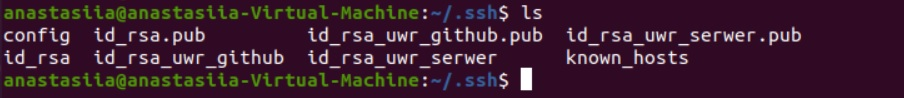
\includegraphics[scale = 0.9]{1.jpg}
    \item Za pomocą ssh-copy-id skopiowałam klucz publiczny na serwer \\
    
    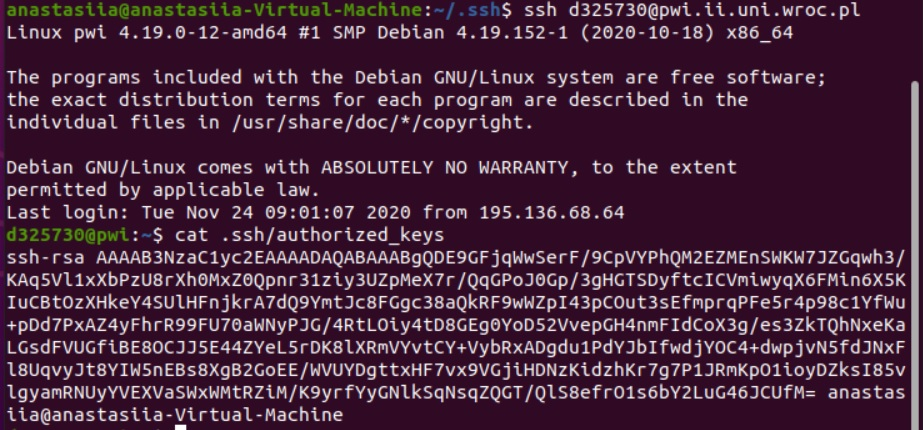
\includegraphics[scale = 0.9]{2.jpg}
    \item Stworzyłam na GitHubie repozytorium PWI-sprawdzian-d325730 i dodałam do niego drugi klucz publiczny \\
    
    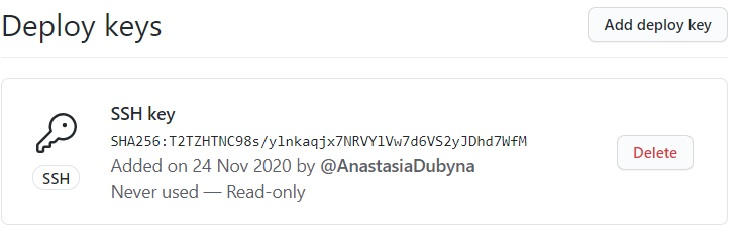
\includegraphics[scale = 0.9]{3.jpg}
    \newpage
    \item Stworzyłam plik konfiguracyjny, który pozwala zalogować się na serwer za pomocą tylko polecenia ssh pwi-sprawdzian\\
    
    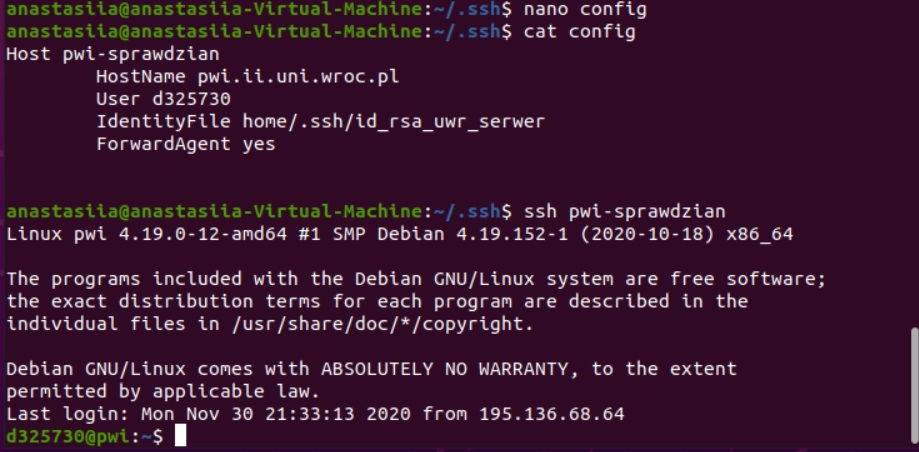
\includegraphics[scale = 0.9]{4.jpg}
    \item W pliku konfiguracyjnym włączyłam ForwardAgent, co pozwala na przekierowanie kluczy lokalnych tak by były dostępne również na serwerze.Tworzenie nowej pary kluczy byłoby rozwiązaniem brzydkim ponieważ wtedy każda osoba która ma dostęp do serwera również będzie miała dostęp do naszego klucza prywatnego. 
\end{enumerate}
\section*{Zadanie III}
\begin{enumerate}
    \item Skopiowałam repozytorium na serwer za pomocą git clone i pobrałam plik ze skosa za pomocą polecenia wget
    Screen nie zawiera tych poleceń, bo to wszystko zrobiłam w trakcie kolokwium i nie widzę potrzeby w ponownym kopiowaniu repozytorium ściągnięciu pliku, żeby to zademonstrować skoro zadanie jest proste\\
    
    
\includegraphics[scale = 0.9]{5.jpg}
    \newpage
    \item Rozpakowałam archiwum za pomocą polecenia tar -xvf \\
    -x: odczytuje podane pliki z archiwum\\
    -v: wyświetla nazwy dołączanych plików \\
    -f: używa archiwum nazwę którego podaliśmy dalej\\
    
    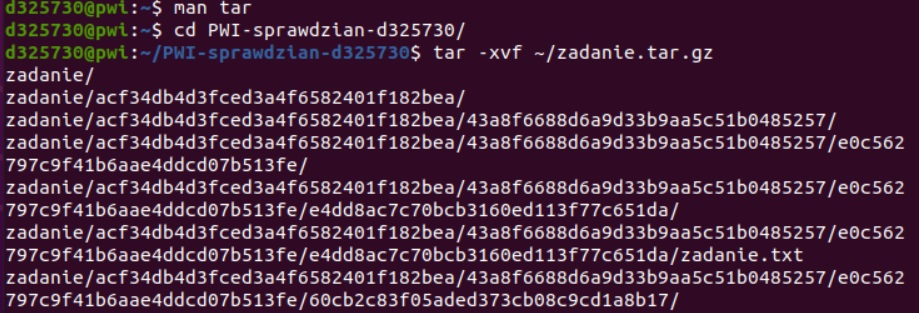
\includegraphics[scale = 0.9]{6.jpg}
    \item Dodałam oraz zakomitowałam zmiany\\
    
    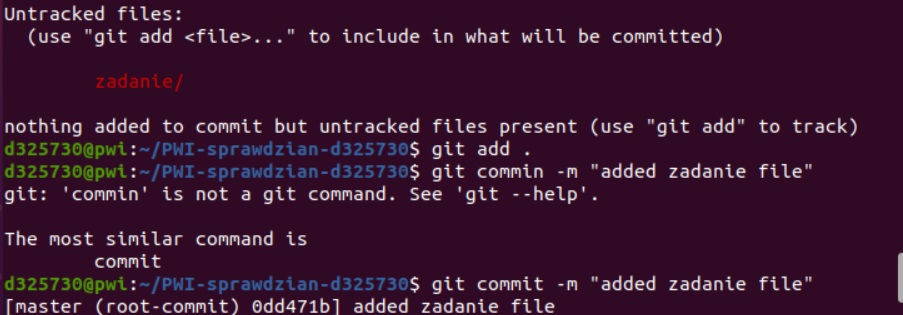
\includegraphics[scale = 0.9]{7.jpg}
    \newpage
    \item Wyliczyłam  MD5 ze stringa d325730 i znalazłam katalog z zadaniem za pomocą polecenia find -name, które poszukuję lokalizację pliku o pewnej nazwie\\
    
    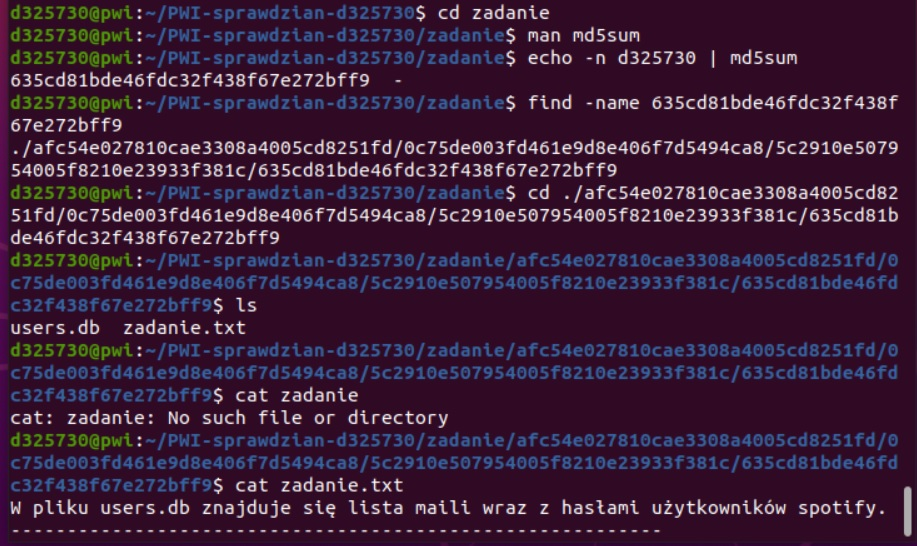
\includegraphics[scale = 0.9]{8.jpg}\\
    \item Znalazłam ile razu w pliku występuję string Country = POLAND za pomocą grep -c (grep do wyszukiwań w tekście oraz -c do obliczenia ilości wyników). Do obliczenia ilości wszystkich użytkowników użyłam najpierw wc -l (liczy ilość wierszy w tekście), a potem grep -c 'Subscription' i grep -c 'Country' (liczy wszystkie wystąpienia słów Subscription oraz Country). Dwie ostatnie liczby są mniejsze o 5 i nie za bardzo wiem, który wynik jest poprawny. Przyjęłam że drugi.  Tak czy owak, nie jest to znaczące dla otrzymanego wyniku - 1.4\% użytkowników z Polski muszą jak najszybciej zmienić swoje hasła 
    
    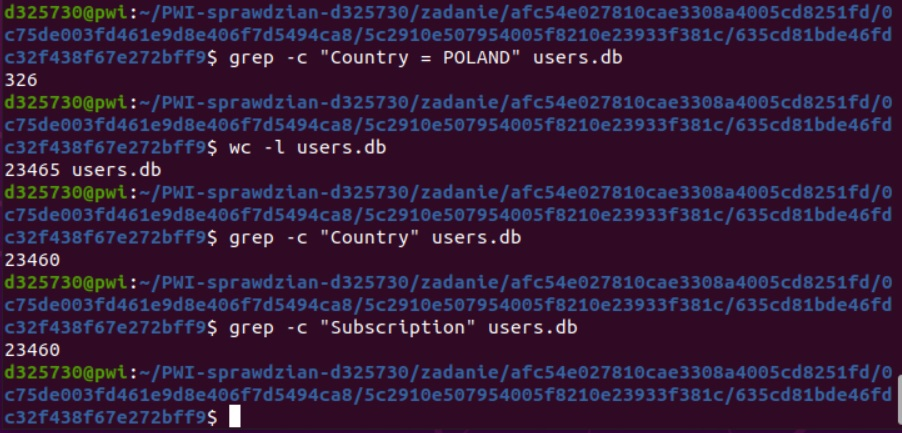
\includegraphics[scale = 0.9]{10.jpg}
    \item Procenty obliczyłam w pythonie\\
    
    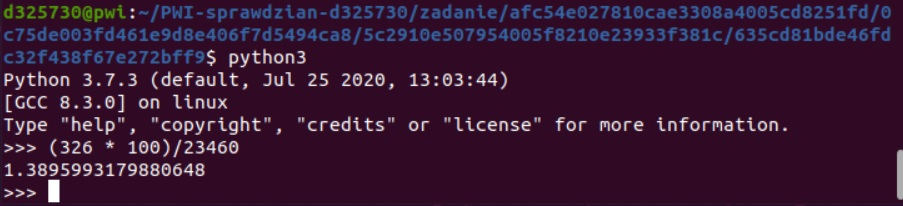
\includegraphics[scale = 0.9]{11.jpg}
    \item W drugiej części zadania użyłam polecenia awk (dzieli każdy wiersz zgodnie z podanym separatorem). W pierwszej części polecenia ze screena dzielę każdy wiersz w pliku przez spacje i dostaję z niego tylko pierwszą kolumnę, która zawiera email użytkownika oraz hasło. W drugiej części z tej kolumny wycinamy tylko hasła przez ":". Wynik zapisujemy do pliku hasła.txt \\
    
    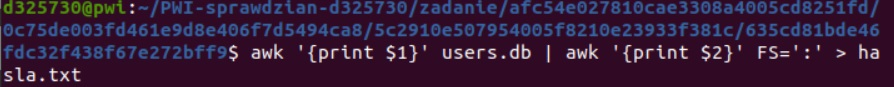
\includegraphics[scale = 0.9]{12.jpg}    
    
\end{enumerate}
\newpage
\section*{Bibliografia}
\begin{itemize}
    \item \url{https://www.youtube.com/watch?v=hQWRp-FdTpc}
    \item \url{https://www.overleaf.com/learn/how-to/How-to_Guides}
    \item \url{https://www.rpi.edu/dept/arc/training/latex/LaTeX_symbols.pdf}
    \item \url{https://www.linux.pl/man/index.php?command=tar}
    \item \url{http://edukacja.3bird.pl/download/informatyka/etap4/gentoo/informatyka-etap4-gentoo-sshd-conf.pdf}
    \item \url{https://www.geeksforgeeks.org/awk-command-unixlinux-examples/}
    \item \url{https://www.cyberciti.biz/faq/howto-use-grep-command-in-linux/}
    
\end{itemize}
\end{document}
